
\documentclass{beamer}
\usetheme{Madrid}

\title[]{Introducción a los modelos climáticos de las fases: CMIP5 y CMIP6}
\author{Marvin J. Quispe Sedano}
\centering
\date{Mayo 2020}

\usepackage{graphicx}


\begin{document}
\maketitle
\begin{frame}{Contenido}
\begin{itemize}
\item ¿Qué es el clima? 
\item ¿Qué son las variables climáticas esenciales?.
\item Tipos de datos climáticos. 
\item Modelos climáticos.
\item CMIP: Coupled Model Intercomparison Project
\item CMIP5 y CMIP6
\end{itemize}
\end{frame}

\begin{frame}{¿Qué es el clima?}
\framesubtitle{¿Todos entendemos verdaderamente lo que significa la palabra clima?}

\begin{itemize}
	\setlength\itemsep{1em}      
    \item La comprensión del clima se basa en observaciones de la atmósfera, los océanos y la superficie terrestre, incluidos los ciclos hidrológicos, del carbono y la criósfera (WMO, 2020).
    \item El clima describe las condiciones del \emph{tiempo meteorológico} promedio, para un lugar en particular y durante un largo periodo de tiempo (WMO, 2020). 
 
\end{itemize}
\end{frame}

\begin{frame}
\frametitle{Clima vs Tiempo atmosférico}
 
\begin{block}{Clima}

Los climatólogos utilizan las normales climáticas (promedios históricos de 30 años de variables como temperatura y precipitación) como puntos de referencia para el estudio del comportamiento de las distintas \emph{variables climáticas} dentro de un contexto histórico (WMO, 2020).

\end{block}
 
\begin{block}{Tiempo atmosférico}
Estudia las condiciones de las variables atmosféricas en periodos de tiempo cortos (minutos a meses) (NASA, 2017).

\end{block}
\end{frame}

\begin{frame}{¿Qué son las variables climáticas esenciales?}
	\begin{itemize}
	\setlength\itemsep{1em}  
	\item Una variable climática esencial (ECV) es una variable física, química 	o biológica o un grupo de variables vinculadas que contribuyen de manera crítica a la caracterización del clima de la Tierra (GCOS, s.f.).   
	\item Las variables climáticas esenciales (ECV's) se identifican según tres criterios: \emph{relevancia, viabilidad y rentabilidad} (GCOS, s.f.).
\end{itemize}
\end{frame}

\begin{frame}{Variables Climáticas Esenciales (ECV)}
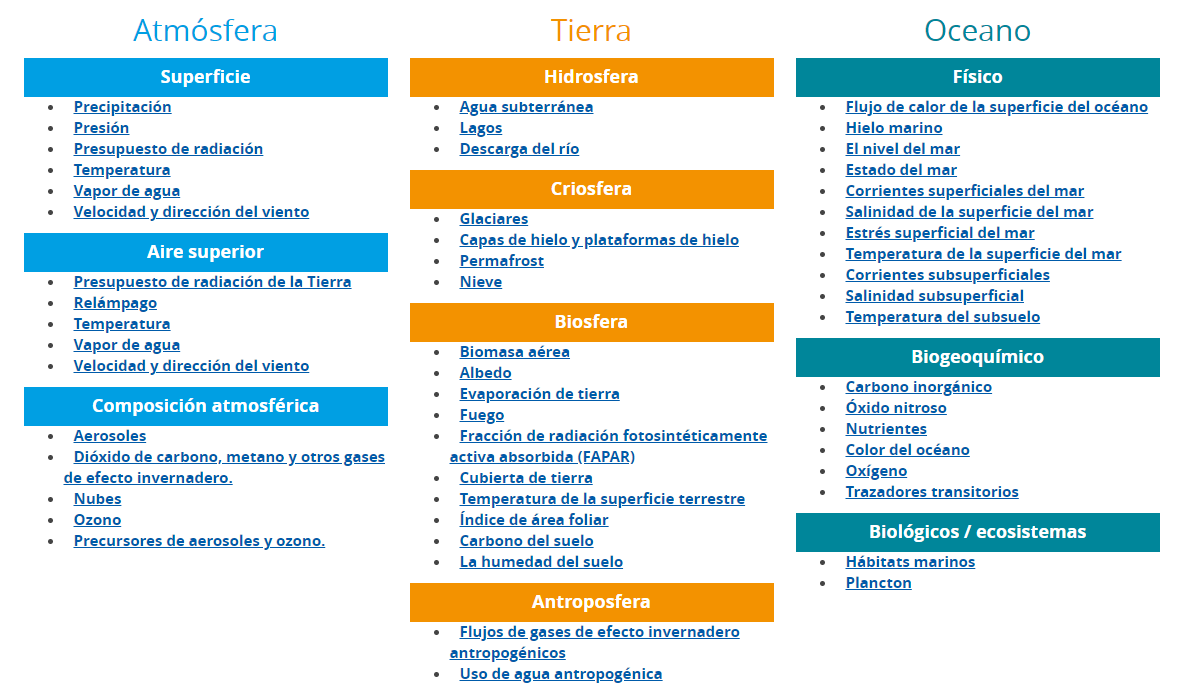
\includegraphics[height=6.8cm]{img/ecv.png}
\centering
\end{frame}

\begin{frame} {Fuentes de datos climáticos}
\framesubtitle{¿Cómo obtenemos datos climáticos?}
 
\begin{block}{Datos observados}

Las observaciones proporcionan información sobre el clima pasado y actual. Hay muchos métodos de observación los cuales se pueden clasificar en \emph{métodos directos e indirectos} (Copernicus, 2019).

\end{block}
 
\begin{block}{Datos modelados}

Un modelo climático es una representación numérica del sistema climático basada en las propiedades físicas, químicas y biológicas de sus componentes, interacciones y procesos de retroalimentación (Copernicus, 2019).

\end{block}
\end{frame}

\begin{frame}{Datos observados directos}
\framesubtitle{in situ}
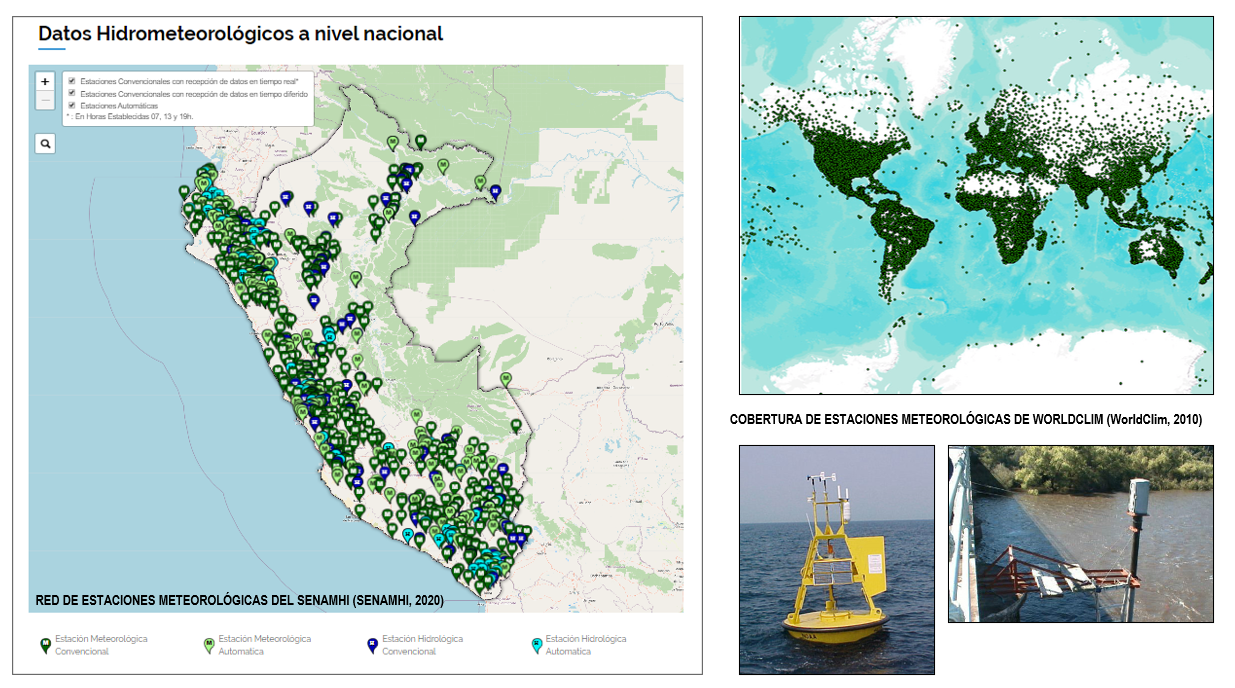
\includegraphics[height=6.8cm]{img/dataobs1.png}
\centering
\end{frame}

\begin{frame}{Datos observados directos}
\framesubtitle{de manera remota}
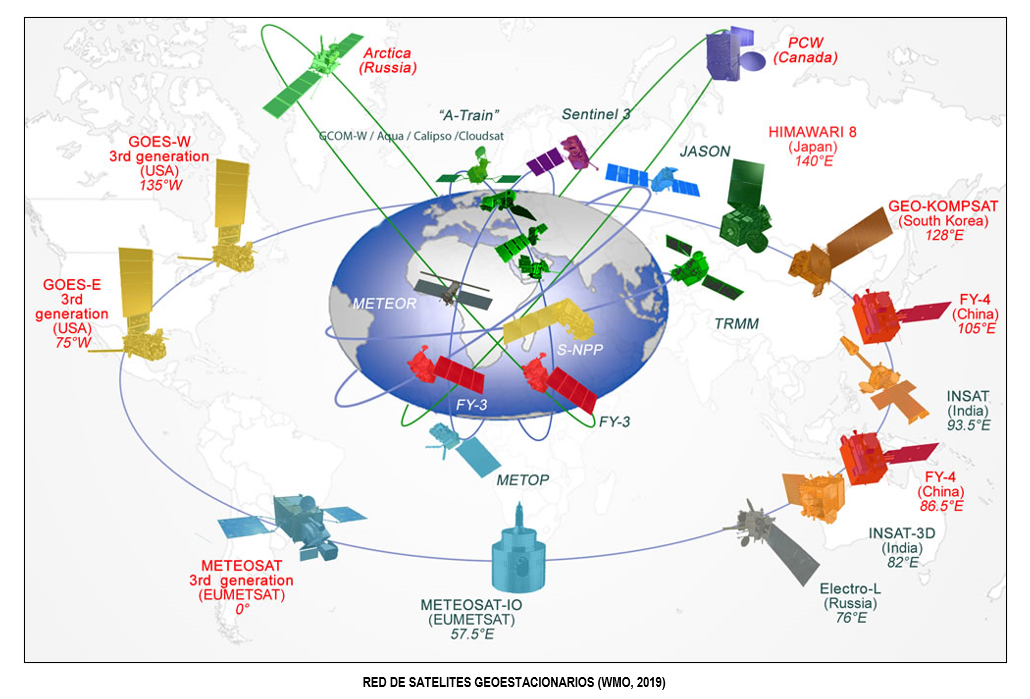
\includegraphics[height=6.8cm]{img/dataobs2.png}
\centering
\end{frame}

\begin{frame}{Datos observados indirectos}
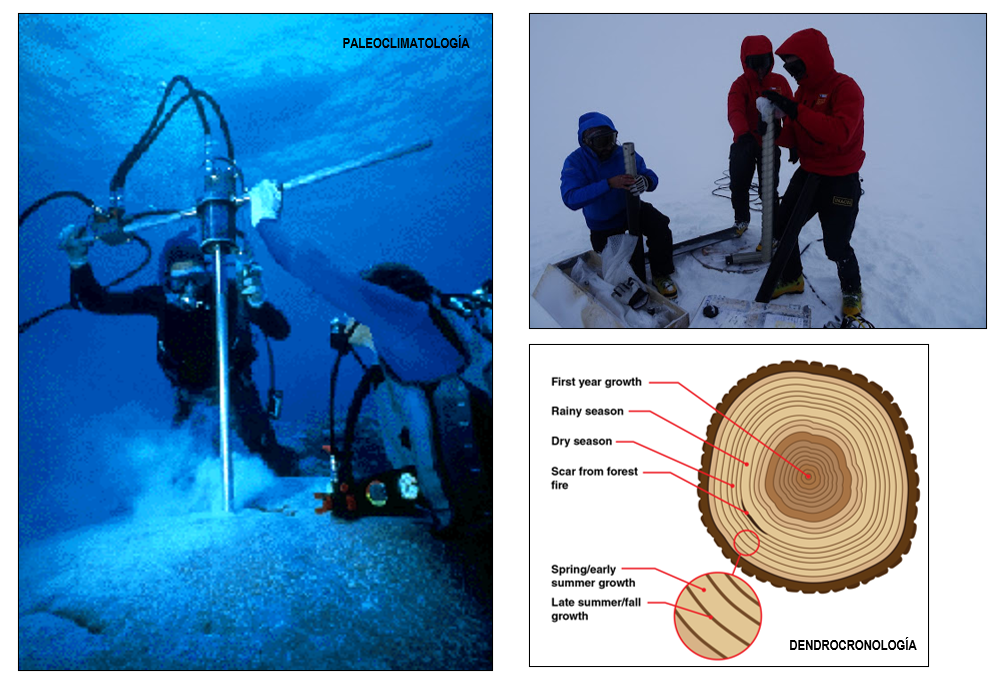
\includegraphics[height=6.8cm]{img/dataind.png}
\centering
\end{frame}

\begin{frame}{Datos observados indirectos}
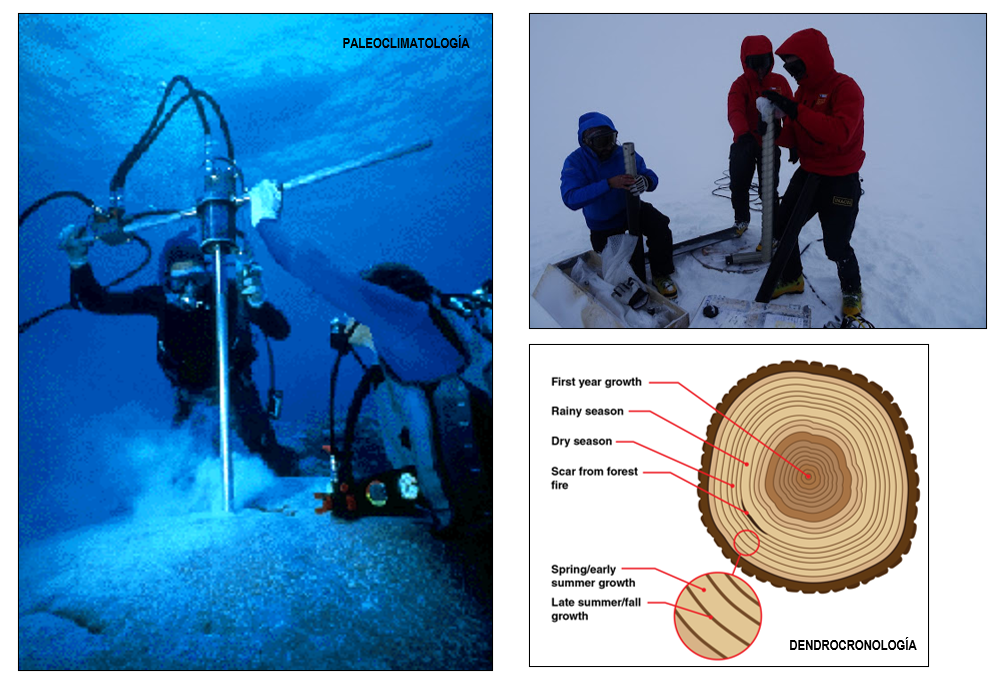
\includegraphics[height=6.8cm]{img/dataind.png}
\centering
\end{frame}

\begin{frame}{Reanálisis}
	\begin{itemize}
	\setlength\itemsep{1em}  
	\item Un reanálisis climático nos proporciona una descripción numérica del clima reciente debido a que es el producto de combinar modelos con observaciones (Copernicus, 2019). 
	\end{itemize}
	\begin{center} 
	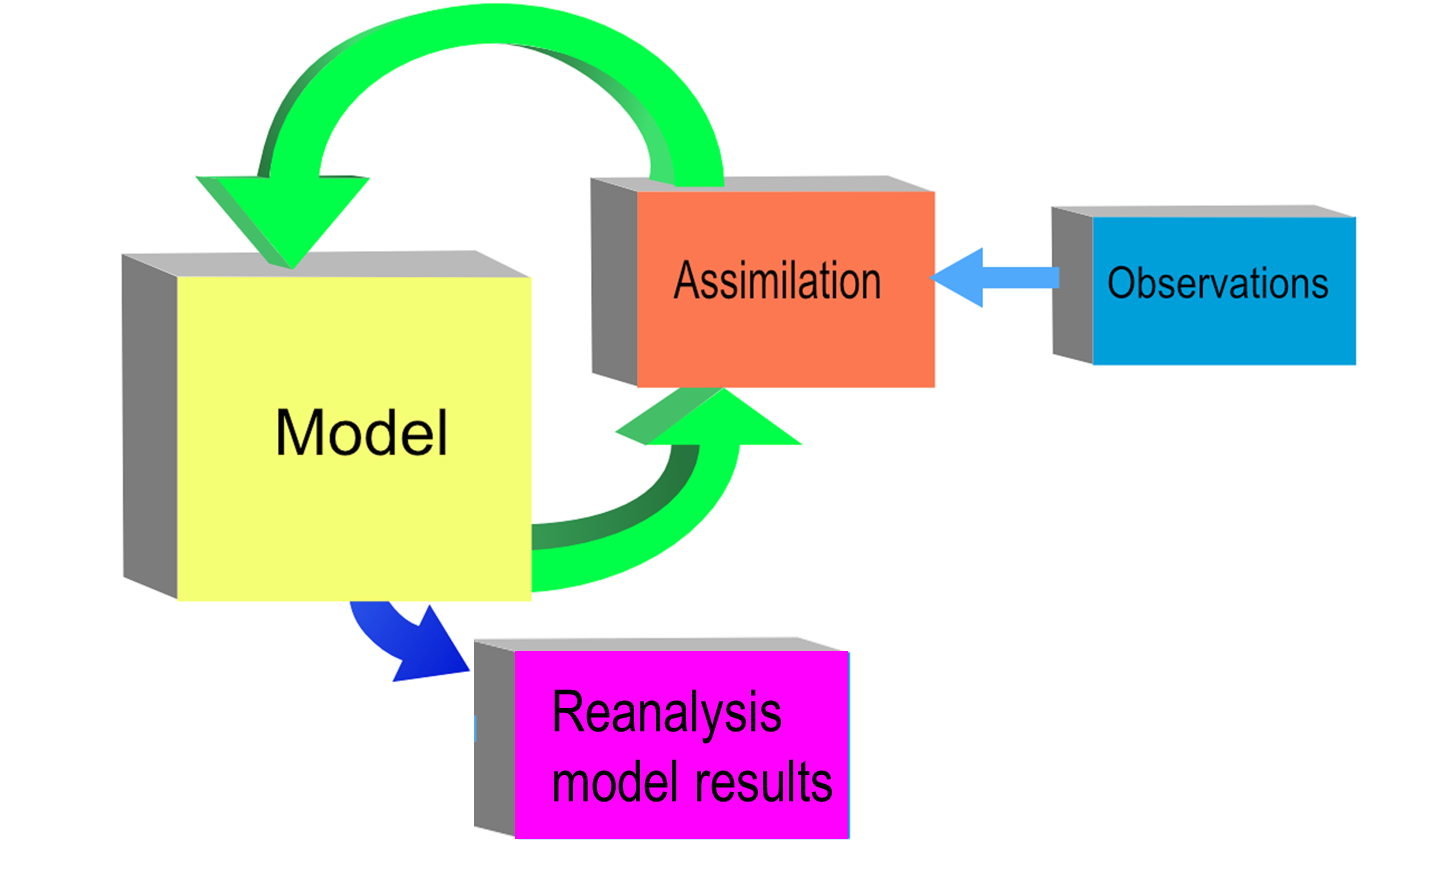
\includegraphics[height=4.8cm]{img/reanalisis.png}
	\end{center}

\end{frame}


\begin{frame}{Modelo climático}
	\begin{itemize}
	\setlength\itemsep{1em}  
	\item Los modelos climáticos se utilizan para determinar cómo cambiarán las condiciones medias y extremas de las variables climáticas (Copernicus, 2019). 
	\item Los modelos climáticos no están tratando de \emph{predecir o pronosticar} lo que va a suceder en un lugar y momento específicos, más bien se utilizan para hacer proyecciones para un futuro (Copernicus, 2019). 
\end{itemize}
	\begin{center} 
	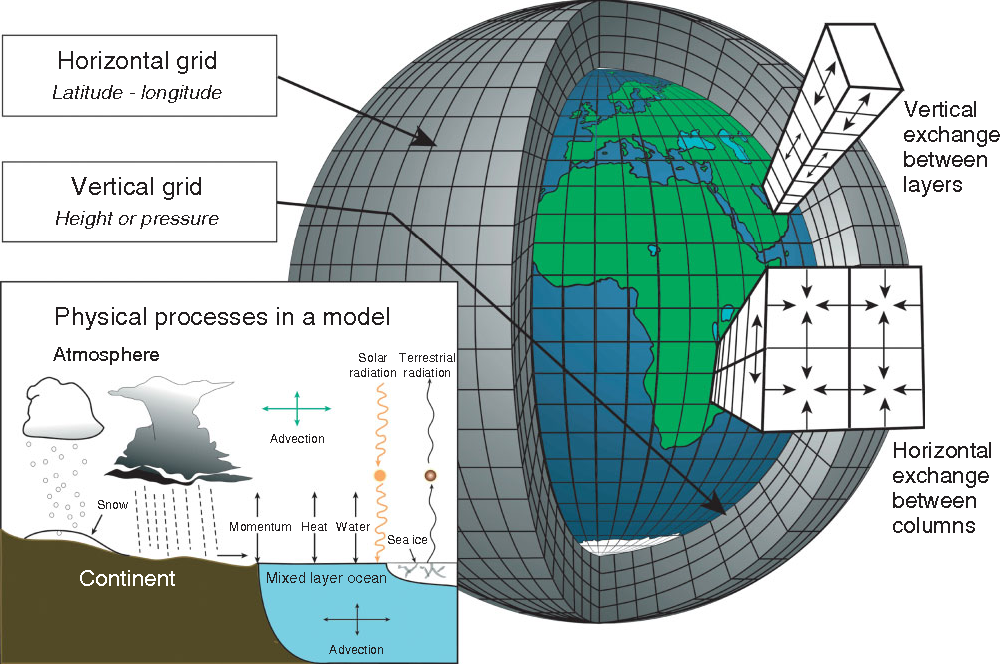
\includegraphics[height=3cm]{img/climmodel.png}
	\end{center}

\end{frame}


\begin{frame} {Tipos de modelos climáticos}
 
\begin{block}{Modelos climáticos globales}
	\begin{itemize}
	\item Modelo global del clima/circulación (GCM)
	\item Modelo del sistema terrestre (ESM)
	\end{itemize}	
\end{block}
 
\begin{block}{Modelos climáticos regionales}
	\begin{itemize}
	\item Modelo regionales de clima (RCM)	
	\end{itemize}
\end{block}

\begin{block}{Modelos de acuerdo a su complejidad}
	\begin{itemize}
	\item Modelo no acoplados (Ejm.- modelos atmosféricos)	
	\item Modelo acoplados (Ejm.- modelos océano-atmosféricos)	
	\end{itemize}
\end{block}

\end{frame}

\begin{frame} {Predicción climática vs Proyección climática}
\framesubtitle{¿Cuál es la diferencia entre el pronóstico del clima y la proyección climática?}

\begin{block}{Predicción climática}
Una predicción o pronostico del clima es un intento de estimar la evolución real del clima natural en el futuro. Pueden realizarse en escalas temporales estacionales, interanuales o de largo plazo (Copernicus, 2019).	
\end{block}

\begin{block}{Proyección climática}
Las proyecciones climáticas dependen de escenarios de emisión/concentración/forzamiento radiativo, que se basan en suposiciones relativas. Por ejemplo, futuros desarrollos socioeconómicos y tecnológicos que pueden realizarse o no, por lo tanto, están sujetos a una gran incertidumbre (Copernicus, 2019).

\end{block}

\end{frame}

\begin{frame} {CMIP: Coupled Model Intercomparison Project}
\framesubtitle {Proyecto de intercomparación de modelos acoplados}
\begin{itemize}
	\setlength\itemsep{1em} 
	\item El objetivo del Proyecto de intercomparación de modelos acoplados (CMIP) es comprender mejor los cambios climáticos pasados, presentes y futuros que surgen de la variabilidad natural no forzada o en respuesta a los cambios en el forzamiento radiativo en un contexto multimodelo (WCRP, 2020). 
	\item El CMIP comenzó en 1995 bajo los auspicios del Grupo de Trabajo sobre Modelado Acoplado (WGCM), el cual pertenece al Programa Mundial de Investigación del Clima (WCRP) (WCRP, 2020). 
	\item El CMIP se ha desarrollado en varias fases, siendo las ultimas fases la quinta (CMIP5) y la sexta (CMIP6). 		
	\end{itemize}
	
\end{frame}

\begin{frame}{Cambios en la complejidad de los modelos climáticos}
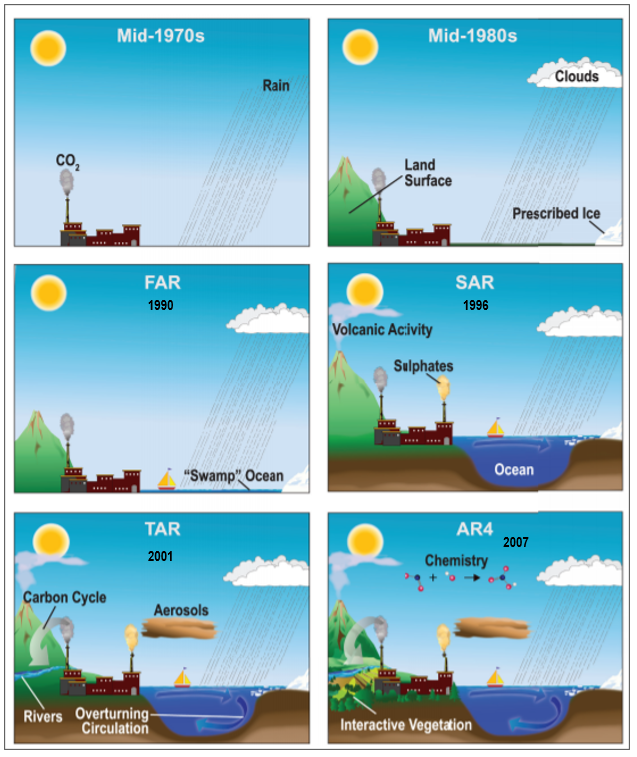
\includegraphics[height=7cm]{img/modelhist.png}
\centering
\end{frame}	
	
\begin{frame}{DECK : Experimentos de diagnóstico, evaluación y caracterización del Klima}
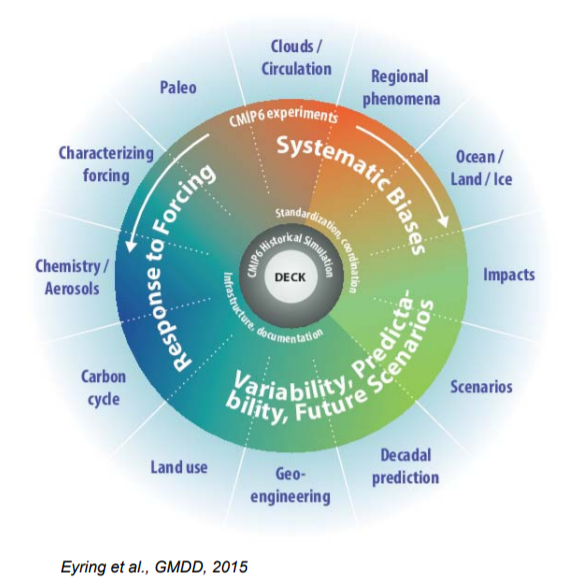
\includegraphics[height=7cm]{img/mips.png}
\centering
\end{frame}	
	
\begin{frame} {Proyecciones climáticas}

\begin{block}{Rutas de Concentración Representativas (RCP)}
\begin{itemize}
	\setlength\itemsep{1em} 
	
	\item El IPCC definió las RCP's para su 5º Informe de evaluación (AR5) en 2014. 

	\item El objetivo de las RCP's es proporcionar descripciones plausibles del futuro, basadas en escenarios socioeconómicos de cómo crece y se desarrolla la sociedad global. 

	\item Los cuatro RCP (a saber, RCP2.6, RCP4.5, RCP6 y RCP8.5) están etiquetados después de un posible rango de valores de forzamiento radiativo en el año 2100 correspondientes a 2.6, 4.5, 6.0 y 8.5 W/m2, respectivamente.
	\end{itemize}	
\end{block}	
\end{frame}	

\begin{frame} {Proyecciones climáticas}

\begin{block}{Rutas Socioeconómicas Compartidas (SSP)}
\begin{itemize}
	\setlength\itemsep{1em} 
	
	\item En los últimos años se han creado una serie de nuevas "rutas" que examinan cómo la sociedad global, la demografía y la economía podrían cambiar en el próximo siglo. Se conocen colectivamente como las "Vías socioeconómicas compartidas" (SSP).


	\end{itemize}	
\end{block}	
\end{frame}	

\begin{frame}{CMIP5 vs CMIP6}
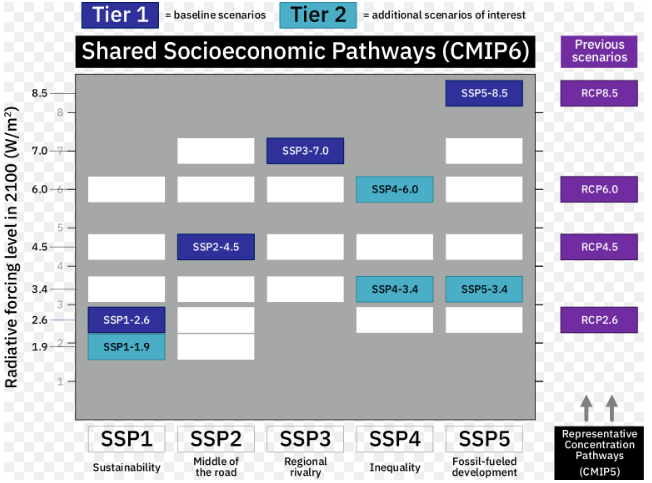
\includegraphics[height=7cm]{img/cmip5y6.png}
\centering
\end{frame}	
	
\begin{frame}{CMIP5 vs CMIP6}
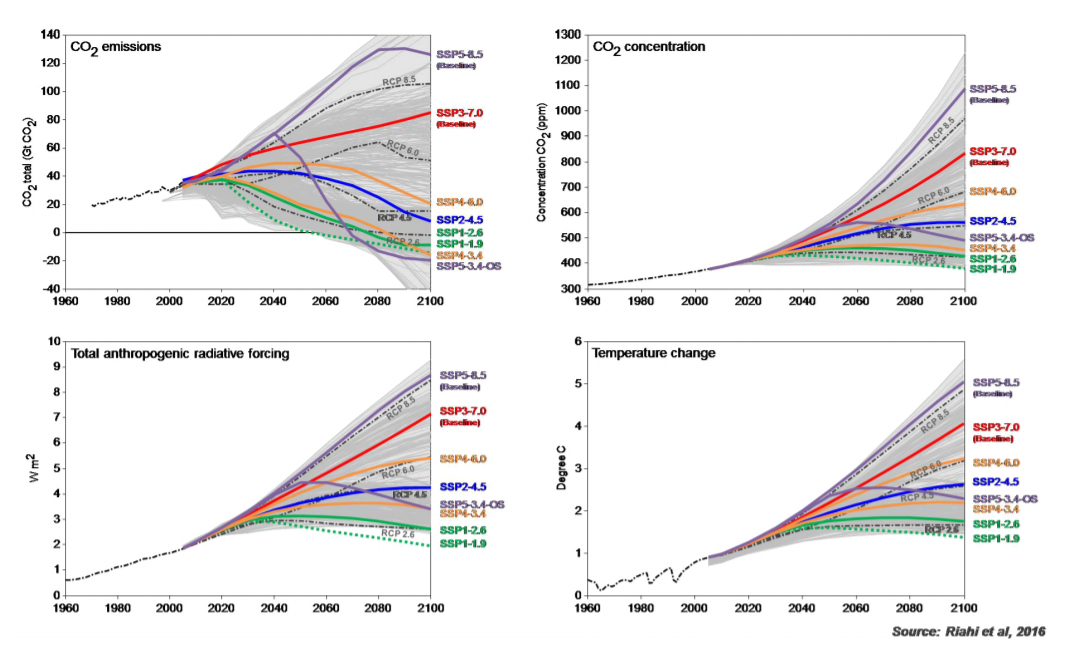
\includegraphics[height=6.5cm]{img/cmip5y6v2.png}
\centering
\end{frame}	

\begin{frame}{CMIP5 vs CMIP6}
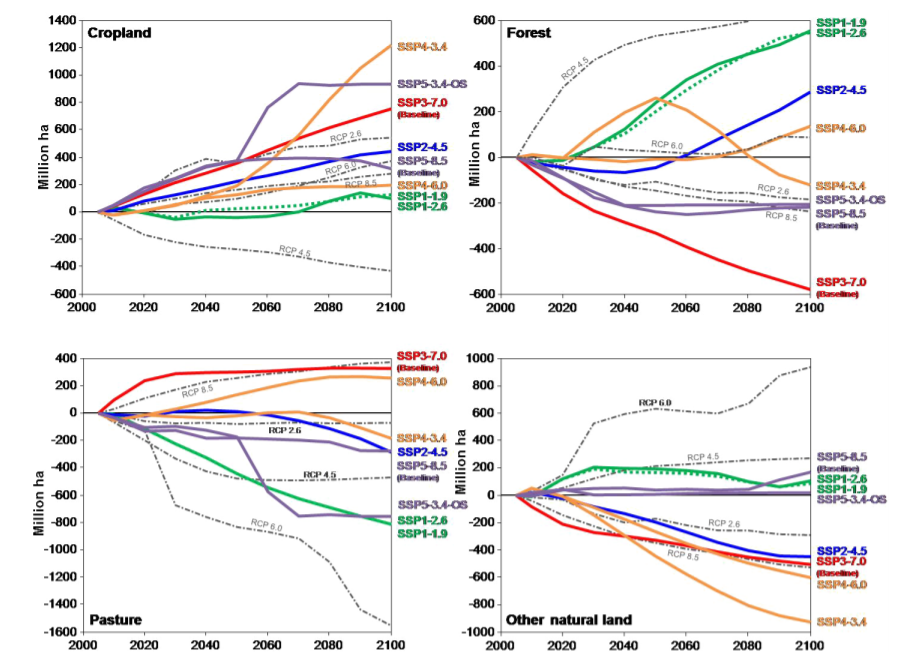
\includegraphics[height=7cm]{img/cmip5y6v3.png}
\centering
\end{frame}	

\begin{frame}
\huge{\centerline{GRACIAS}}
\end{frame}

\end{document}